\documentclass[acmsmall,screen,nonacm]{acmart}
\raggedbottom
\usepackage{eso-pic}
\usepackage{silence}
\WarningFilter{latex}{Command \showhyphens has changed}

\AtBeginDocument{%
  \providecommand\BibTeX{{Bib\TeX}}}

\title{Pneumonia Classification from Pediatric Chest X-Rays with Lightweight Deep Learning Models}
\author{Carolina Reis}
\email{luanacarolina@ua.pt}
\affiliation{%
  \institution{University of Aveiro}
  \city{Aveiro}
  \country{Portugal}}
  
\author{Jakub Błaszczyk}
\email{jakub.blaszczyk@ua.pt}
\affiliation{%
  \institution{University of Aveiro}
  \city{Aveiro}
  \country{Portugal}}
  \affiliation{%
  \institution{Lodz University of Technology}
  \city{Lodz}
  \country{Poland}}

\renewcommand{\shortauthors}{Reis and Błaszczyk}
\settopmatter{printacmref=false}

\begin{document}

\AddToShipoutPictureBG*{%
  \AtPageUpperLeft{%
    \raisebox{-1.2cm}[0pt][0pt]{%
      \makebox[0pt][l]{%
        \hspace*{0.9cm}
\includegraphics[width=2.6cm]{logo-ua}%
      }%
      \makebox[\paperwidth][r]{%
        
\includegraphics[width=3.3cm]{logo-deti}\hspace*{0.9cm}%
      }%
    }%
  }%
}

\begin{abstract}
This project proposes a lightweight deep learning pipeline for classifying pediatric chest X-rays as normal or pneumonia. We used the public Chest X-Ray Images (Pneumonia) dataset, which contains 5,863 labeled images with an imbalanced train/validation/test split. Our methodology compares a small custom CNN baseline against transfer learning with ResNet18 and DenseNet121, and uses Grad-CAM for qualitative inspection of model attention. Evaluation will focus on accuracy, precision, recall, F1-score, AUROC, and inference time, with special emphasis on pneumonia recall because false negatives are clinically costly.
\end{abstract}

%%
%% The code below follows the ACM CCS structure used in the template.
%%
\begin{CCSXML}
<ccs2012>
 <concept>
  <concept_id>10010147.10010257</concept_id>
  <concept_desc>Computing methodologies~Machine learning</concept_desc>
  <concept_significance>300</concept_significance>
 </concept>
 <concept>
  <concept_id>10010147.10010178.10010224.10010225</concept_id>
  <concept_desc>Computing methodologies~Computer vision tasks</concept_desc>
  <concept_significance>300</concept_significance>
 </concept>
 <concept>
  <concept_id>10010405.10010444</concept_id>
  <concept_desc>Applied computing~Life and medical sciences</concept_desc>
  <concept_significance>100</concept_significance>
 </concept>
</ccs2012>
\end{CCSXML}

\ccsdesc[300]{Computing methodologies~Machine learning}
\ccsdesc[300]{Computing methodologies~Computer vision tasks}
\ccsdesc[100]{Applied computing~Life and medical sciences}

\keywords{pneumonia detection, chest X-rays, transfer learning, Grad-CAM}

\begin{teaserfigure}
  \centering
  \captionsetup{justification=centering}
  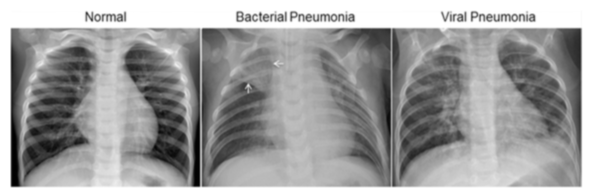
\includegraphics[width=0.72\textwidth]{pneumonia}
  \caption{Examples shown in the dataset overview: a normal chest X-ray, bacterial pneumonia, and viral pneumonia.}
  \Description{A horizontal teaser image with three chest X-ray examples corresponding to normal, bacterial pneumonia, and viral pneumonia, matching the illustration shown in the dataset overview on Kaggle.}
\end{teaserfigure}

\maketitle

\section{Problem Statement}

\subsection{Background and Motivation}
Pneumonia is a life-threatening respiratory infection that affects millions of people worldwide each year, disproportionately impacting young children and elderly patients, especially in low-resource settings. Timely and accurate diagnosis is critical, yet it depends heavily on the availability of trained radiologists, a resource that remains scarce in many hospitals. Chest X-ray imaging is one of the most accessible diagnostic tools for detecting pneumonia, which makes it a natural target for automated analysis. A model that can distinguish between normal and pneumonia chest X-rays may help clinicians by flagging suspicious cases, reducing diagnostic delays, and acting as a second-opinion tool in resource-constrained environments.

\subsection{Project Goal and Scope}
The goal of this project is to train and evaluate a binary image classifier that receives a single chest X-ray as input and outputs the probability of the \textit{PNEUMONIA} class rather than the \textit{NORMAL} class. The scope includes data preparation, a lightweight CNN baseline, fine-tuning pretrained models, and Grad-CAM inspection. Out of scope are multi-label thoracic diagnosis, pneumonia subtype identification, lesion segmentation, severity grading, and any real clinical deployment without external validation.

\subsection{Expected Contribution}
This project is expected to provide a compact benchmark for pneumonia classification on pediatric chest X-rays, centered on the trade-off between accuracy, recall, interpretability, and computational cost. By comparing a custom CNN baseline with lightweight transfer-learning models and complementing quantitative results with Grad-CAM visual inspection, we aim to identify the most reasonable level of model complexity for this dataset.

\section{Dataset}

\subsection{Source and Access}
The dataset used in this project is the \textit{Chest X-Ray Images (Pneumonia)} dataset, originally curated by Kermany et al.~\cite{kermany2018} and publicly distributed on Kaggle~\cite{kagglechestxray}. It is publicly accessible and requires no special approval; downloading requires a free Kaggle account. The images are organized into pre-split train, validation, and test folders, which makes it straightforward to integrate into a standard deep learning workflow. Before training, the images still require resizing, normalization, and conversion to a format compatible with pretrained models.

\subsection{Size and Label Structure}
The Kaggle version contains 5,863 pediatric chest X-ray images labeled for a binary classification task with two outputs: \textit{NORMAL} and \textit{PNEUMONIA}. The split is strongly imbalanced, especially in training, with 1,341 normal and 3,875 pneumonia images; the validation set contains only 8 normal and 8 pneumonia images, and the test set contains 234 normal and 390 pneumonia images. The samples are chest radiographs stored as JPEG images with varying original resolutions, so resizing is required before training and accuracy alone is not enough to characterize performance.

\subsection{Preprocessing}
Images will be resized to $224 \times 224$ pixels to match the input requirements of ResNet18 and DenseNet121, and to keep memory usage manageable. Pixel values will be normalized using ImageNet mean and standard deviation (mean = [0.485, 0.456, 0.406], std = [0.229, 0.224, 0.225]), since we plan to use pretrained weights. Because the original dataset is grayscale X-rays saved as JPEG, images will be converted to three-channel RGB by replicating the single channel. For the training split, we will apply light data augmentation, including random horizontal flips and small random rotations (up to  $\pm 10^\circ$) to improve generalization. The provided train/val/test split will be used as-is, with no additional samples filtered out, unless corrupted files are found during initial inspection.

\subsection{Sample Data}
A typical sample is a frontal pediatric chest radiograph in grayscale showing the lungs, heart silhouette, ribs, and occasional text markers. Normal cases usually have clearer lung fields, while pneumonia cases may present focal or diffuse opacities, although some examples are visually subtle and overlap with normal-looking patterns.

\section{Methodology}

\subsection{Baseline Approach}
The baseline will be a small custom CNN composed of three convolutional blocks, each including a Conv2D layer, batch normalization, ReLU activation, and max pooling, followed by global average pooling and a single fully connected output layer with sigmoid activation for binary classification. This architecture has no pretrained components, is fast to train on modest hardware, and provides a meaningful lower-bound reference point against which the transfer-learning models can be compared. Binary cross-entropy will be used as the loss function, and the model will be trained for up to 20 epochs with early stopping based on validation loss.

\subsection{Proposed Model}
Our main model will be DenseNet121~\cite{huang2017densenet}, initialized with ImageNet weights and adapted for binary classification with a single sigmoid output. DenseNet is a good fit because its dense connectivity encourages feature reuse, keeps the number of parameters manageable, and has shown strong performance in chest radiography settings such as CheXNet~\cite{rajpurkar2017chexnet}. In parallel, we will also fine-tune ResNet18~\cite{he2016resnet} as a lighter comparison with lower inference cost. Both models can be trained on a single Colab GPU while still leaving room for error analysis and Grad-CAM-based interpretability~\cite{selvaraju2017gradcam}.

\subsection{Training Setup}
Both the baseline and transfer-learning models will be trained using the Adam optimizer with an initial learning rate of $10^{-4}$, reduced on plateau by a factor of 0.5 after 3 stagnant epochs. Binary cross-entropy will be used as the loss function throughout. Training will run for up to 30 epochs with early stopping (patience 5) to prevent overfitting, using a batch size of 32. For the pretrained models (ResNet18/DenseNet121), we will apply a two-phase strategy: first training only the final classification head for 5 epochs, then unfreezing the full network for fine-tuning. Experiments will be run on a single GPU (Google Colab T4 or equivalent), which is sufficient given the dataset size and model scale.

\subsection{Architecture Diagram}
\begin{figure}[h]
  \centering
  \resizebox{\linewidth}{!}{%
    \begin{tabular}{c@{\hspace{0.15cm}}c@{\hspace{0.15cm}}c@{\hspace{0.15cm}}c@{\hspace{0.15cm}}c@{\hspace{0.15cm}}c@{\hspace{0.15cm}}c@{\hspace{0.15cm}}c@{\hspace{0.15cm}}c}
      \fbox{\parbox[c][1.5cm][c]{1.9cm}{\centering Chest\\X-ray\\image}} &
      $\rightarrow$ &
      \fbox{\parbox[c][1.5cm][c]{2.2cm}{\centering Resize\\Normalize\\RGB conversion}} &
      $\rightarrow$ &
      \fbox{\parbox[c][1.8cm][c]{2.7cm}{\centering Feature extractor\\Custom CNN /\\ResNet18 /\\DenseNet121}} &
      $\rightarrow$ &
      \fbox{\parbox[c][1.5cm][c]{1.8cm}{\centering Sigmoid\\output}} &
      $\rightarrow$ &
      \fbox{\parbox[c][1.8cm][c]{2.0cm}{\centering Metrics\\and\\Grad-CAM}}
    \end{tabular}%
  }
  \caption{Proposed training and evaluation pipeline.}
  \Description{A pipeline diagram showing chest X-ray input, preprocessing, model backbone, binary output, and evaluation with metrics and Grad-CAM.}
\end{figure}

\section{Evaluation Plan}

\subsection{Metrics}
The primary evaluation metrics will be accuracy, precision, recall (sensitivity), F1-score, and AUROC. Given the clinical context, recall for the pneumonia class is of particular importance, since a false negative (missed pneumonia) is more harmful than a false positive. We will therefore report per-class recall explicitly and monitor it as a key metric alongside macro-F1. Inference time per image will also be measured to compare models in terms of efficiency, which is relevant for potential deployment in resource-limited settings.

\subsection{Baselines and Comparisons}
The main comparison will involve three systems trained under the same protocol: the custom CNN baseline, ResNet18, and DenseNet121. This setup compares a model trained from scratch against two transfer-learning alternatives with different complexity-efficiency trade-offs. We will also include a small ablation on data augmentation for the best pretrained model. Grad-CAM will be used as a qualitative sanity check to verify whether the models focus on plausible lung regions instead of spurious artifacts.

\subsection{Experimental Protocol}
All models will be evaluated on the same fixed train/validation/test split provided with the Kermany dataset. No test data will be used during training or hyperparameter selection. Hyperparameters such as learning rate, batch size, and augmentation strategy will be selected from validation performance only, after which the best configuration for each model will be evaluated once on the test set. Each model will be trained with three random seeds to assess result stability, and we will report mean and standard deviation across runs. All experiments will be conducted in a shared Colab notebook to ensure reproducibility.

\subsection{Success Criteria}
We will consider the project successful if at least one transfer-learning model clearly outperforms the custom CNN baseline on macro-F1 and AUROC while maintaining strong recall for pneumonia cases. A second criterion is reaching pneumonia recall above 0.90 on the fixed test set. Beyond raw metrics, a successful result should include a reproducible pipeline and Grad-CAM visualizations that attend mostly to lung regions rather than corners, labels, or acquisition artifacts.

\section{Ethics and Limitations}

\subsection{Potential Biases}
The Kermany dataset was collected from pediatric patients at Guangzhou Women and Children's Medical Center, which introduces a substantial demographic limitation: the model is trained and evaluated on a single population, institution, and age group, and may not generalize to adult patients or images acquired with different X-ray equipment or protocols. Class imbalance is also present in the training set, with pneumonia samples outnumbering normal ones; this may push the model toward over-predicting pneumonia, artificially inflating recall while reducing precision. In addition, chest X-ray classifiers are known to exploit spurious correlations such as medical device artifacts or text annotations rather than true pathological patterns — a risk we will partially address through Grad-CAM inspection.

\subsection{Limitations of the Approach}
This approach has several technical limitations. The dataset is relatively small and imbalanced for a medical imaging problem, and the validation split is extremely small, which makes model selection noisy. The task is also simplified to binary normal-versus-pneumonia classification, whereas real clinical workflows involve multiple thoracic conditions and uncertain cases. In addition, our experiments rely on a single public dataset with no external validation, so good in-dataset performance may not transfer to other hospitals, imaging protocols, or adult populations.

\subsection{Responsible Use}
The resulting model should be used only as an educational prototype or as a decision-support aid under clinician supervision, never as a stand-alone diagnostic or triage system. Predictions from a model trained on a single pediatric dataset are not sufficient to confirm or exclude pneumonia in real patients, and false negatives may delay necessary treatment. Any real deployment would require external multi-site validation, calibration, bias assessment, clinical oversight, and the appropriate ethical and regulatory approvals.

\bibliographystyle{ACM-Reference-Format}
\bibliography{ProjectProposalReport}

\end{document}
